% Couverture Thèse TPT Latex v2
% Fabrice Linot 04/12/11 

\documentclass[11pt,a4paper]{book}
\usepackage[left=1.3cm,top=0cm,right=1.3cm,bottom=1.2cm]{geometry}
\usepackage{graphicx}
\usepackage{eso-pic}
\usepackage{array}
\usepackage[french]{babel}
\usepackage[utf8x]{inputenc}
\usepackage[T1]{fontenc}
\usepackage{textcomp}
\usepackage{helvet}	% or \usepackage{lmodern}
\renewcommand\textnumero{n$^{\textsf{{\tiny O}}}$}
\renewcommand{\familydefault}{\sfdefault}

\usepackage{ifpdf}
\newcommand\BackgroundPic{
\ifpdf
	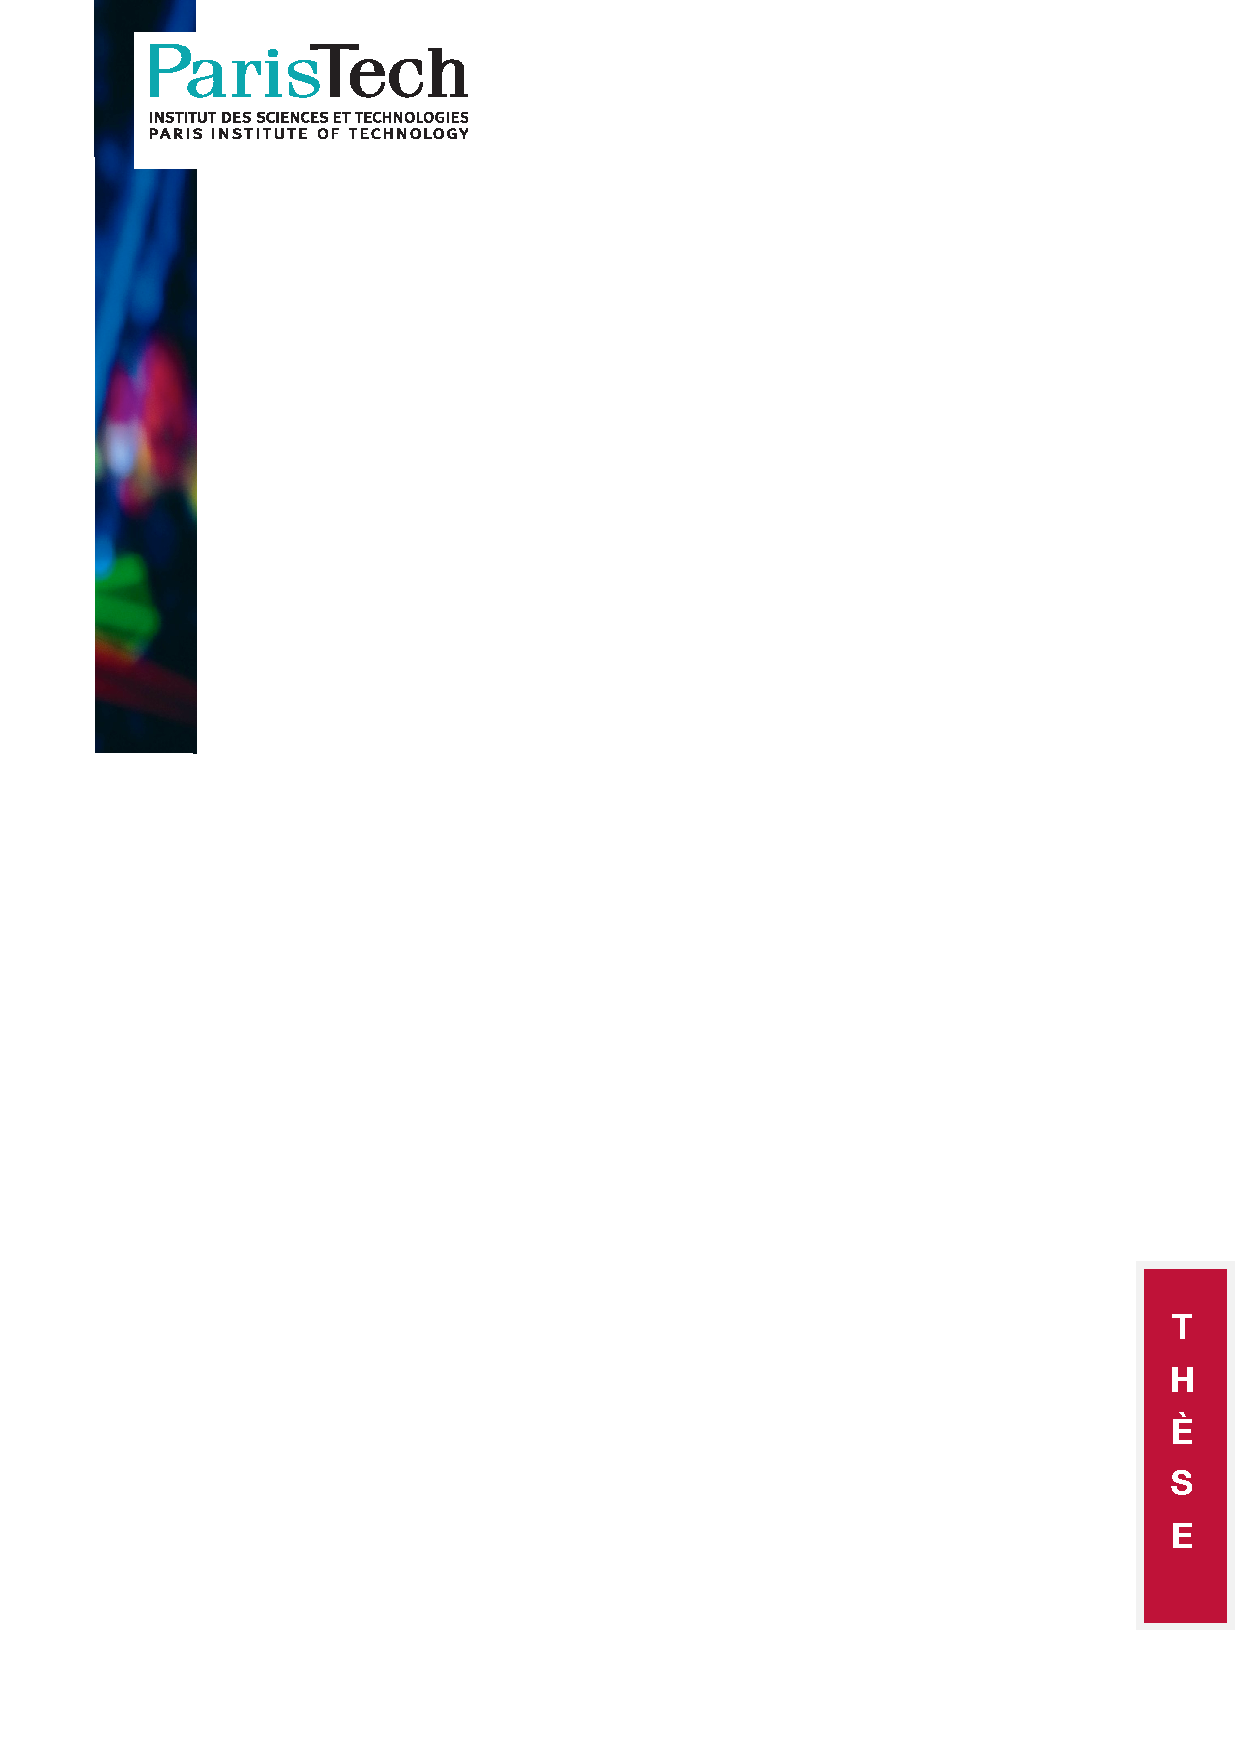
\includegraphics[height=\paperheight,width=\paperwidth]{cover_bg}
\else
	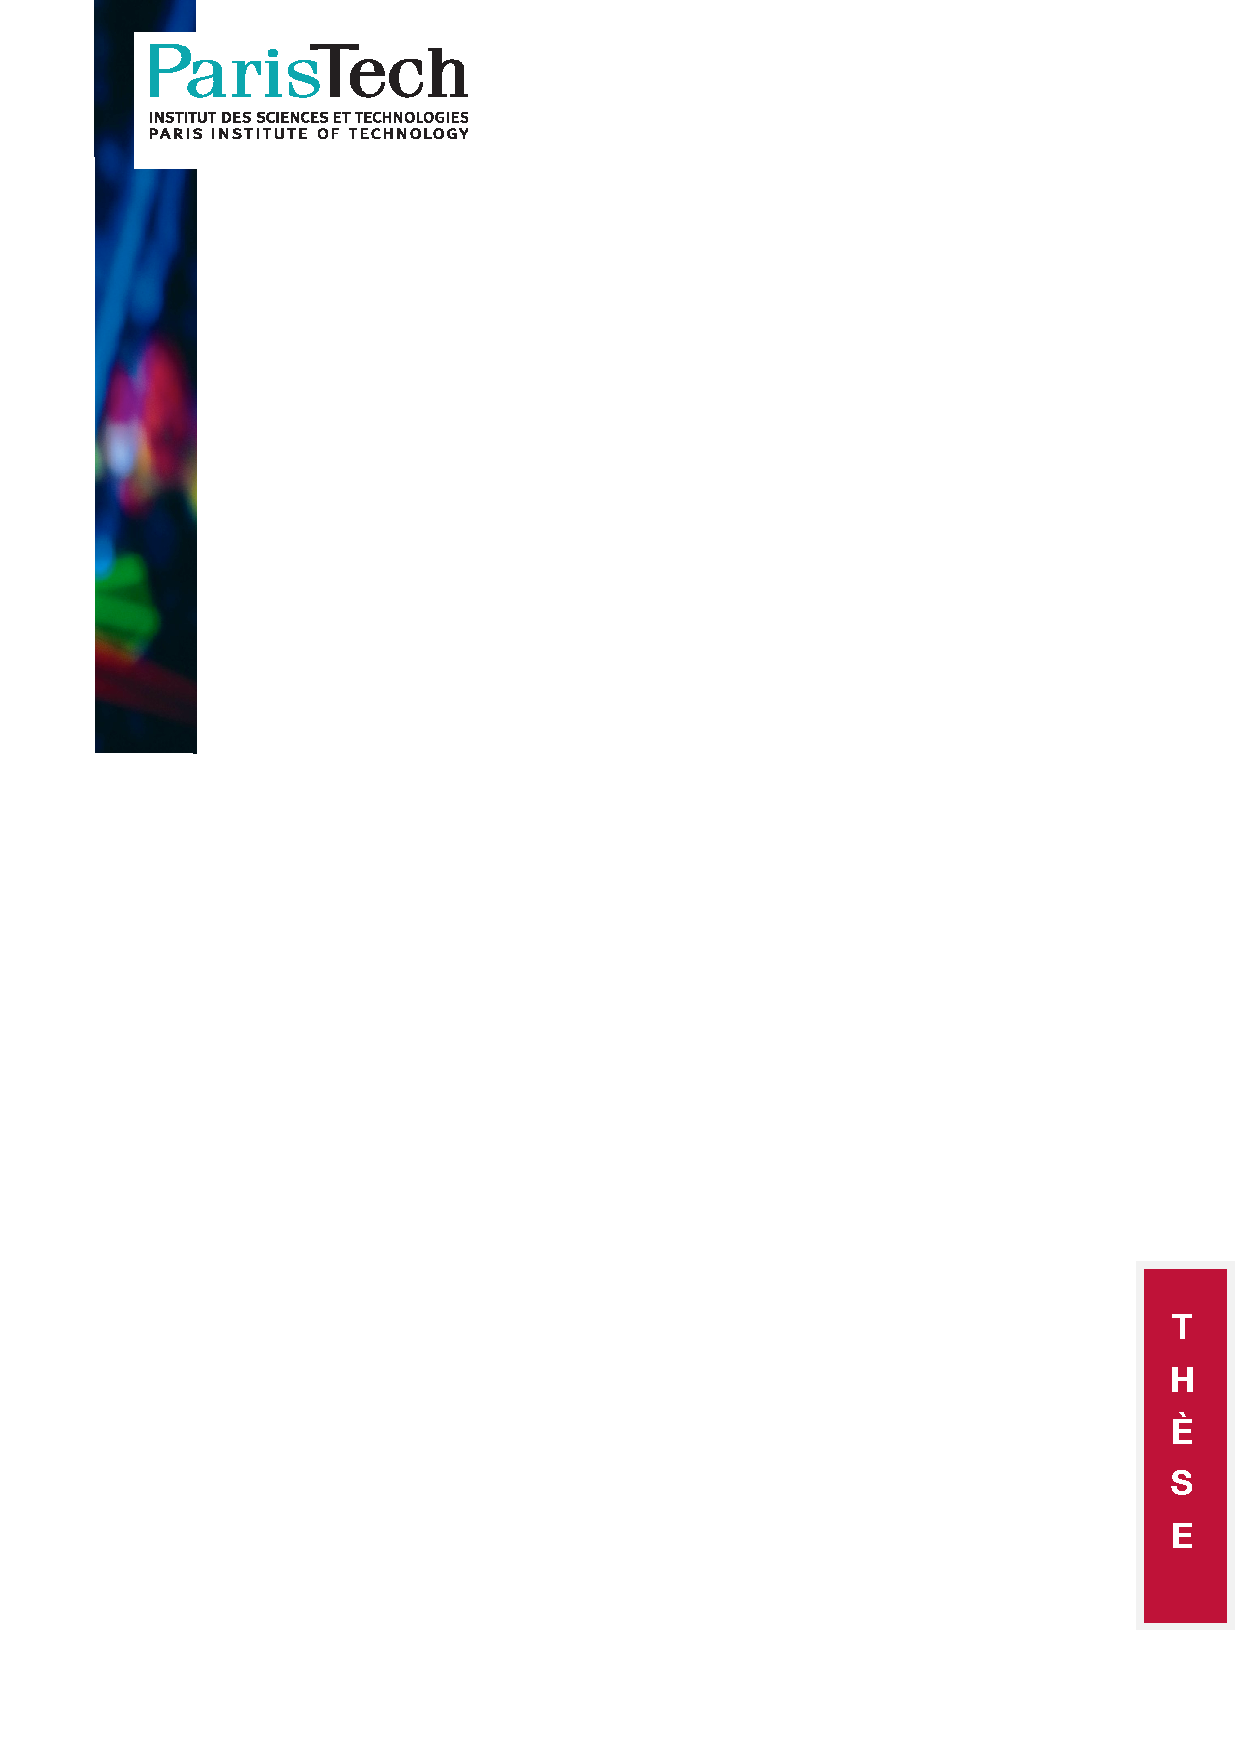
\includegraphics[height=\paperheight,width=\paperwidth]{cover_bg}
\fi
}

\pagestyle{empty}

\begin{document}
\AddToShipoutPicture*{\BackgroundPic}
~


\begin{flushright}


\includegraphics[width=90px]{telecom}

%?
{\small {2017-ENST-0060~~~~}}
\end{flushright}



%\vspace{0.cm}
\begin{center}
%



\includegraphics[scale=0.65]{edite} \\
%{\small {EDITE - ED 130}}


%
\vspace{.5cm}
%
%
%
%{\Large École doctorale \textnumero XX: texte}\\		% version une ligne
%{\Large École doctorale \textnumero XX:\\ texte}\\		% version deux lignes (changer les espaces en conséquence
%
%
%
\vspace{1.0cm}
%
%
%
{\LARGE {\bf Doctorat ParisTech}}\\
\vspace{1.1cm}
{\LARGE {\bf T H \`{E} S E}}\\
\vspace{0.5cm}
{\normalsize {\bf pour obtenir le grade de docteur d\'{e}livr\'{e} par}}\\
%
%
%
\vspace{.9cm}
%
%
%
%
{\LARGE {\bf TELECOM ParisTech}}\\
\vspace{0.6cm}
{\Large {\bf Sp\'{e}cialit\'{e} - Informatique et R\'{e}seaux }}\\
%
%
%
\vspace{.8cm}
%
%
%
{\normalsize {\it pr\'{e}sent\'{e}e et soutenue publiquement par}}\\
\vspace{0.7cm}
{\Large {\bf Wenqin Shao}}\\
\vspace{0.24cm}
{\normalsize le 29/11/2017}\\
%
%
%
\vfill
%
%
%
\textcolor[RGB]{191,18,56}{
\noindent
\LARGE {\bf Ing\'{e}nierie du Trafic Inter-domaine Bas\'{e}e sur la Mesure}
}
%
%
%
\vfill
%
%
%
{\normalsize
\begin{tabular}{c}
Directeur de th\`{e}se:					{\bf Jean-Louis Rougier}\\
Co-encadrement de th\`{e}se:		{\bf Luigi Iannone }
\end{tabular}
}
\end{center}
%
%
%
\vfill
%
%
%
\flushleft
\begin{minipage}{.91\textwidth}	% ou .91\textwidth si vous n'avez pas assez de place
{\bf Jury}\\
{\bf M. Philippe Owezarski}, {\small Directeur de recherche, LAAS - CNRS}
	\hfill Rapporteur\\
{\bf M. Chadi Barakat}, {\small Chargé de Recherche HDR, INRIA, Sophia Antipolis - Méditerranée}
	\hfill Rapporteur\\
{\bf Mme. Cristel Pelsser}, {\small Professeur, Université de Strasbourg - CNRS}
	\hfill Examinateur\\
{\bf Mme. Sandrine Vaton}, {\small Professeur, Telecom Bretagne}
	\hfill Examinateur\\
{\bf M. François Devienne}, {\small Co-foundateur, BORDER 6}
	\hfill Invit\'{e}\\
{\bf M. Luigi Iannone}, {\small Maître de conf\'{e}rences, Telecom Paristech}
	\hfill Directeur de th\`{e}se\\
{\bf M. Jean-Louis Rougier}, {\small Professeur, Telecom Paristech}
	\hfill Directeur de th\`{e}se\\

%{\bf Mme/M. Prénom NOM}, {\small Titre, Unité de recherche, Ecole}
%	\hfill Fonction\\
%{\bf Mme/M. Prénom NOM}, {\small Titre, Unité de recherche, Ecole}
%	\hfill Fonction\\
\end{minipage}\\
%
%
%
%\vspace{-.1cm}
%
%
%
\centering
{\bf TELECOM ParisTech}\\
{\small école de l'Institut Télécom - membre de ParisTech}
%
%
%
\end{document}
